%!TEX program = xelatex
\documentclass[xcolor=table,aspectratio=169,11pt]{beamer}
\usepackage[utf8]{inputenc}
\usepackage[spanish]{babel}
\usepackage{graphicx}
\usepackage{tikz}
\usepackage{enumitem}
\usepackage{fontawesome5}

% Paquetes necesarios
\usepackage{tikz}
\usetikzlibrary{positioning, shadows.blur}  % Para posicionamiento relativo y sombras

% Definir colores personalizados (puedes cambiarlos PARA TICKS)
\definecolor{azulclaro}{RGB}{220, 240, 255}   % Fondo claro
\definecolor{azulborde}{RGB}{100, 150, 220}   % Borde más oscuro
\definecolor{azulfuerte}{RGB}{0, 80, 160}     % Texto o énfasis

% Paquetes recomendados (cárgalos después de la clase)
\usepackage{booktabs}          % Para \toprule, \midrule, \bottomrule (más elegantes)
\usepackage{array}             % Mejora columnas p{}
\usepackage{ragged2e}          % Para justificar texto en columnas p{}
\usepackage{xcolor}            % Ya viene cargado por beamer, pero lo dejamos por si acaso

% Colores personalizados (ajusta según tu gusto)
\definecolor{azulencabezado}{RGB}{30, 80, 140}
\definecolor{grisclaro}{RGB}{245, 245, 245}

\usepackage{tikz}
\usetikzlibrary{positioning, shadows.blur, arrows.meta}

% Colores (ajusta según tu tema si usas uno personalizado)
\definecolor{azulclaro}{RGB}{220, 240, 255}
\definecolor{azuloscuro}{RGB}{30, 80, 140}
\definecolor{grisazul}{RGB}{100, 140, 180}


% Tema moderno
\usetheme{Madrid}
\usecolortheme{whale}

\usepackage{background}

% Configuración de la marca de agua (logo tenue en esquina inferior derecha)
\backgroundsetup{
	scale=0.45,                % Tamaño más grande para que se note en el centro (prueba 0.35 a 0.55)
	angle=0,                   % Sin rotación (o pon 15 o -15 si quieres un efecto diagonal sutil)
	opacity=0.08,              % Muy tenue (0.06–0.12 para que no moleste el texto)
	contents={
\includegraphics[height=16cm]{cau-logo.png}},  % Aumenta height para mayor visibilidad
	position=current page.center,   % ← ¡CENTRO DE LA PÁGINA!
	% No necesitas vshift ni hshift cuando usas .center
}

% Esto es clave: fuerza que el fondo se aplique en la capa correcta de Beamer
\setbeamertemplate{background}{\BgMaterial}

% Colores personalizados
\definecolor{azuloscuro}{RGB}{0,51,102}
\definecolor{azulclaro}{RGB}{51,102,153}
\definecolor{gris}{RGB}{102,102,102}

\setbeamercolor{structure}{fg=azuloscuro}
\setbeamercolor{title}{fg=white,bg=azuloscuro}
\setbeamercolor{frametitle}{fg=white,bg=azuloscuro}

% Información del documento
\title{Elaboración de Monografía}
\subtitle{Sesión 1:  Estructura y Tipos de Monografías}
\author{CAU - UNSCH | Edison Achalma }
\date{\today}

\begin{document}
	
	% Portada
	\begin{frame}
		\titlepage
	\end{frame}
	
	% Índice
	\begin{frame}{Contenido de la Sesión}
		\tableofcontents
	\end{frame}
	
	% ============== SESIÓN 1: 1.5 HORAS ==============
	\section{Primera Parte}
	
	\subsection{¿Qué es una Monografía?}
	
	\begin{frame}{Etimología y Definición}
		\begin{block}{Origen del término}
			\textbf{Monografía} proviene del griego:
			\begin{itemize}
				\item \textit{Monos} = Uno
				\item \textit{Graphos/Graphein} = Escritura o describir
			\end{itemize}
		\end{block}
		
		\vspace{0.5cm}
		
		\begin{alertblock}{Definición formal}
			Documento expositivo y explicativo que aborda un tema específico de manera \textbf{exhaustiva, sistemática y metódica}.
		\end{alertblock}
	\end{frame}
	
	\begin{frame}{Características Fundamentales}
		\begin{columns}[T]
			\column{0.5\textwidth}
			\textbf{Una monografía es:}
			\begin{itemize}
				\item Estudio \textbf{profundo} de un tema único
				\item Análisis \textbf{riguroso} y fundamentado
				\item Organización \textbf{sistemática} de información
				\item Contribución al \textbf{conocimiento}
			\end{itemize}
			
			\column{0.5\textwidth}
			\textbf{Una monografía NO es:}
			\begin{itemize}
				\item Un simple resumen de información
				\item Una opinión personal sin respaldo
				\item Un trabajo superficial
				\item Un ensayo literario
			\end{itemize}
		\end{columns}
	\end{frame}
	
\begin{frame}{Diferencias entre Monografía, Ensayo y Tesis}
	\centering
	\vspace{0.3cm}
	
	\begin{table}
		\footnotesize   % Tamaño más legible que \tiny
		
		\rowcolors{2}{grisclaro!50}{white}  % Alternancia sutil de fondo en filas
		
		\begin{tabular}{>{\RaggedRight}p{2.6cm}>{\RaggedRight}p{3.6cm}>{\RaggedRight}p{3.6cm}>{\RaggedRight}p{3.6cm}}
			
			\toprule
			\rowcolor{azulencabezado!20}
			\textbf{Característica} & \textbf{Monografía} & \textbf{Ensayo} & \textbf{Tesis} \\
			\midrule
			
			Objetivo 
			& Organizar y sintetizar información existente 
			& Argumentar una postura personal 
			& Aportar conocimiento original \\
			
			\midrule
			Extensión 
			& Media (20--50 páginas) 
			& Corta (5--15 páginas) 
			& Extensa (80--200+ páginas) \\
			
			\midrule
			Rigor metodológico 
			& Alto 
			& Medio a variable 
			& Muy alto \\
			
			\midrule
			Originalidad 
			& Puede incluirla 
			& No es requisito 
			& Indispensable \\
			
			\midrule
			Estructura 
			& Rígida y formal 
			& Flexible 
			& Muy estructurada \\
			
			\bottomrule
		\end{tabular}
		
	\end{table}
	
	\vspace{0.4cm}
	\scriptsize Fuente: Elaboración propia basada en criterios académicos estándar.
	\end{frame}
	
	\subsection{Tipos de Monografías}
	
\begin{frame}{Clasificación según Enfoque y Metodología}
	\centering
	
	\begin{tikzpicture}[
		node distance = 0.25cm and 0.1cm,          % Espacio horizontal y vertical
		every node/.style = {
			rectangle,
			rounded corners=4pt,
			draw=azulborde,
			thick,
			fill=azulclaro,
			text width=4.8cm,                       % Anchura fija para uniformidad
			minimum height=2.6cm,                   % Altura mínima
			align=center,
			font=\bfseries\small,
			drop shadow={shadow xshift=2pt, shadow yshift=-2pt, opacity=0.25}
		}
		]
		
		% Nodo 1 - Izquierda
		\node (compilacion) 
		{\textbf{MONOGRAFÍA DE COMPILACIÓN}\\[0.4em]
			Recopila, organiza y analiza \\
			información existente sobre un tema \\
			(COMPILACIÓN = CURADOR)};
		
		% Nodo 2 - Centro
		\node[right=of compilacion] (investigacion)
		{\textbf{MONOGRAFÍA DE INVESTIGACIÓN}\\[0.4em]
			Investigación original, \\
			aporta nuevos datos o interpretaciones \\
			(INVESTIGACIÓN = EXPLORADOR)};
		
		% Nodo 3 - Derecha
		\node[right=of investigacion] (experiencias)
		{\textbf{MONOGRAFÍA DE ANÁLISIS DE EXPERIENCIAS}\\[0.4em]
			Basada en vivencias prácticas o casos \\
			(ANÁLISIS = PRÁCTICA + TEORÍA)};
		
	\end{tikzpicture}
	
	\vspace{0.5cm}
	\small{Clasificación común según enfoque metodológico}
\end{frame}
	
	\begin{frame}{Tipo 1: Monografía de Compilación}
		\begin{block}{Definición}
			El investigador actúa como \textbf{curador de conocimiento}, analizando críticamente la bibliografía existente.
		\end{block}
		
		\textbf{Características:}
		\begin{itemize}
			\item Síntesis de fuentes existentes
			\item Análisis crítico de la literatura
			\item Organización coherente de información
			\item Identificación de vacíos y tendencias
		\end{itemize}
		
		\vspace{0.3cm}
		\textbf{Ejemplo:} \textit{"Enfoques pedagógicos en la enseñanza de matemáticas: Una revisión de la literatura 2015-2025"}
	\end{frame}
	
	\begin{frame}{Tipo 2: Monografía de Investigación}
		\begin{block}{Definición}
			Se enfoca en temas \textbf{nuevos o poco explorados}, realizando investigación original con datos propios.
		\end{block}
		
		\textbf{Características:}
		\begin{itemize}
			\item Recolección de datos primarios
			\item Aplicación de metodologías específicas
			\item Análisis original de resultados
			\item Contribución al conocimiento del área
		\end{itemize}
		
		\vspace{0.3cm}
		\textbf{Ejemplo:} \textit{"Impacto del uso de ChatGPT en el rendimiento académico de estudiantes universitarios: Estudio experimental"}
	\end{frame}
	
	\begin{frame}{Tipo 3: Monografía de Análisis de Experiencias}
		\begin{block}{Definición}
			Común en carreras prácticas. Consiste en el estudio directo de una \textbf{realidad concreta} comparada con casos semejantes.
		\end{block}
		
		\textbf{Características:}
		\begin{itemize}
			\item Reflexión crítica sobre práctica profesional
			\item Comparación con casos similares
			\item Conclusiones basadas en experiencia
			\item Aplicación de teoría a la práctica
		\end{itemize}
		
		\vspace{0.3cm}
		\textbf{Ejemplo:} \textit{"Implementación de metodologías ágiles en startups peruanas: Análisis de tres casos"}
	\end{frame}
	
	\subsection{Estructura Estándar de una Monografía}
	
	\begin{frame}{Estructura de una Monografía (PRÁCTICA EN WORD)}
		\begin{columns}[T]
			% Columna izquierda: Imagen (mantiene el tamaño)
			\column{0.48\textwidth}
			\centering
			\vspace{0.3cm}
			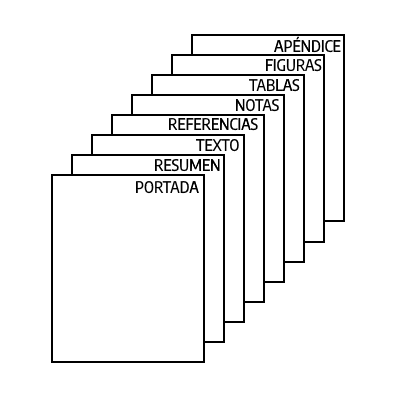
\includegraphics[width=\textwidth,height=0.85\textheight,keepaspectratio]{estructura-monografia-diagrama.png}
			\vspace{0.4cm}
			\small Esquema general de la estructura típica de una monografía
			
			% Columna derecha: Texto más compacto
			\column{0.52\textwidth}
			\footnotesize  % ← Reduce el tamaño de fuente aquí (o usa \small si es muy pequeño)
			\vspace{0.2cm}  % Menos espacio arriba
			
			\textbf{Elementos Preliminares:}
			\begin{enumerate}[noitemsep,topsep=2pt]  % Reduce espaciado entre ítems
				\item Portada
				\item Resumen/Abstract (opcional)
				\item Índice
			\end{enumerate}
			
			\vspace{0.2cm}
			\textbf{Cuerpo Principal:}
			\begin{enumerate}[resume*]  % Continúa la numeración anterior
				\item Introducción
				\item Marco Teórico
				\item Metodología (si aplica)
			\end{enumerate}
			
			\vspace{0.2cm}
			\textbf{Desarrollo y Cierre:}
			\begin{enumerate}[resume*]
				\item Resultados y Análisis
				\item Discusión
				\item Conclusiones
			\end{enumerate}
			
			\vspace{0.2cm}
			\textbf{Soportes Documentales:}
			\begin{enumerate}[resume*]
				\item Referencias Bibliográficas
				\item Apéndices (si aplica)
			\end{enumerate}
		\end{columns}
	\end{frame}

\begin{frame}{1. Portada: La Carta de Presentación (PRÁCTICA EN WORD)}
	\begin{columns}[T]  % T = alineación superior
		% Columna izquierda: Imagen de portada de monografía
		\column{0.48\textwidth}
		\centering
		\vspace{0.5cm}
		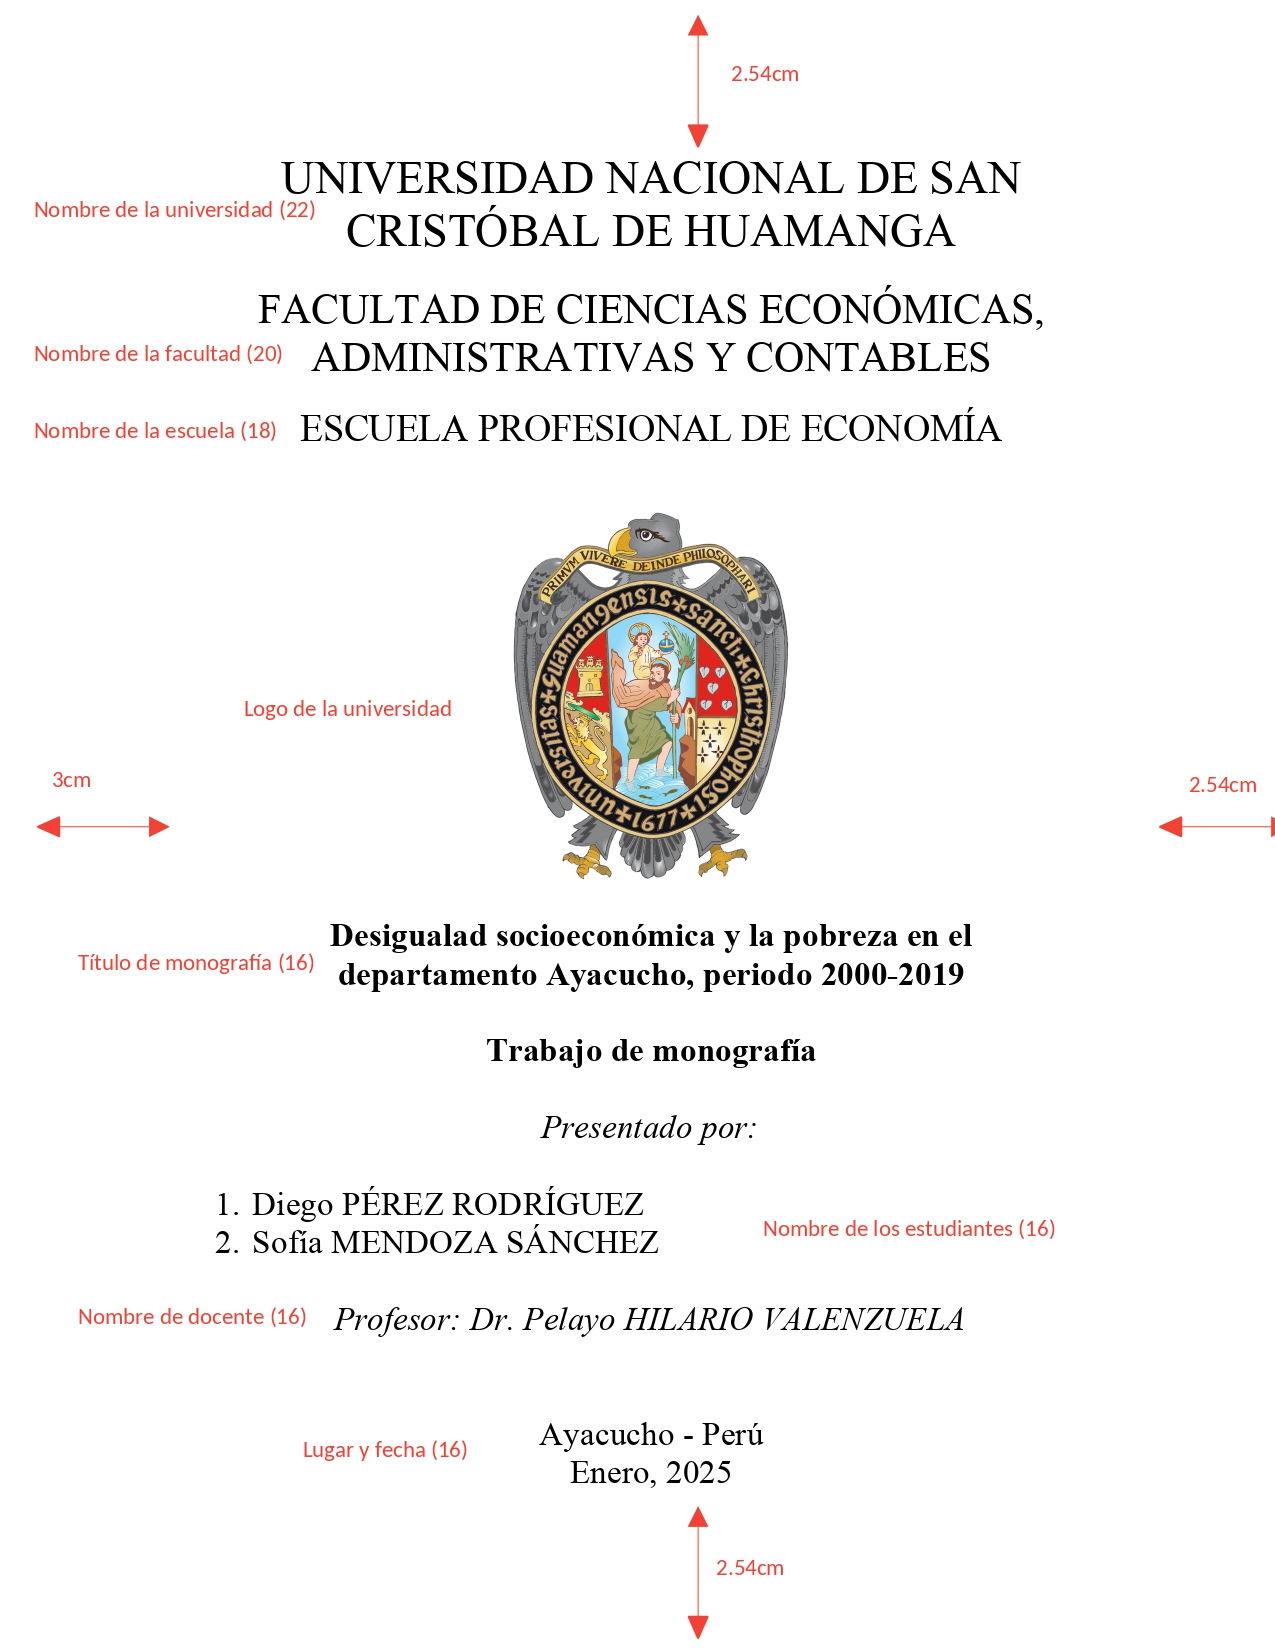
\includegraphics[width=\textwidth,height=0.85\textheight,keepaspectratio]{portada-monografia-ejemplo.jpg}
		% ↑ Cambia "portada-monografia-ejemplo.jpg" por el nombre real de tu imagen
		% Opcional: agrega un pequeño pie de foto
		\vspace{0.3cm}
		\small Ejemplo de portada de monografía académica
		
		% Columna derecha: Lista de elementos obligatorios
		\column{0.52\textwidth}
		\vspace{0.8cm}
		\textbf{Elementos obligatorios:}
		\begin{itemize}
			\item Nombre de la institución
			\item Título del trabajo (máximo 20 palabras)
			\item Nombre del autor
			\item Nombre del tutor/asesor
			\item Ciudad y fecha
		\end{itemize}
		
		\vspace{0.6cm}
		\begin{alertblock}{Importante}
			El título debe ser \textbf{informativo, atractivo y conciso}. Evitar frases como "Estudio sobre..." o "Investigación de..."
		\end{alertblock}
	\end{columns}
\end{frame}
	
	\begin{frame}{2-3. Resumen e Índice}
		\begin{block}{Resumen/Abstract (150-250 palabras)}
			Síntesis que incluye: objetivo, metodología, resultados principales y conclusiones.
		\end{block}
		
		\vspace{0.3cm}
		
		\begin{block}{Índice}
			Listado organizado y numerado de todas las secciones con sus respectivas páginas. Obligatorio en documentos extensos.
		\end{block}
	\end{frame}
	
	\begin{frame}{4. Introducción: Enganchando al Lector}
		\begin{alertblock}{La página más importante}
			Debe presentar el panorama completo de la investigación y motivar la lectura.
		\end{alertblock}
		
		\textbf{Contenidos esenciales:}
		\begin{enumerate}
			\item Oración gancho inicial
			\item Presentación del tema
			\item Problemática o pregunta de investigación
			\item Objetivos (general y específicos)
			\item Justificación de la importancia
			\item Metodología empleada
			\item Estructura del documento
		\end{enumerate}
	\end{frame}
	
	% ============== SESIÓN 2: 1.5 HORAS ==============
	\section{Segunda Parte}
	
	\subsection{Estructura Estándar (continuación)}
	
	\begin{frame}{5. Marco Teórico / Revisión de Literatura}
		\begin{block}{Propósito}
			Fundamentar teóricamente la investigación y demostrar conocimiento del estado del arte.
		\end{block}
		
		\textbf{Contenido:}
		\begin{itemize}
			\item Conceptos fundamentales
			\item Teorías relevantes
			\item Antecedentes de investigación
			\item Variables y definiciones operacionales
		\end{itemize}
		
		\vspace{0.3cm}
		\textbf{Extensión:} Aproximadamente 20-30\% del documento total
	\end{frame}
	
	\begin{frame}{6-8. Metodología, Resultados y Discusión}
		\begin{columns}[T]
			\column{0.33\textwidth}
			\textbf{Metodología}
			\begin{itemize}
				\item Tipo de estudio
				\item Población/muestra
				\item Instrumentos
				\item Procedimientos
			\end{itemize}
			
			\column{0.33\textwidth}
			\textbf{Resultados}
			\begin{itemize}
				\item Presentación objetiva
				\item Tablas y figuras
				\item Análisis descriptivo
			\end{itemize}
			
			\column{0.33\textwidth}
			\textbf{Discusión}
			\begin{itemize}
				\item Interpretación
				\item Comparación con literatura
				\item Limitaciones
			\end{itemize}
		\end{columns}
	\end{frame}
	
	\begin{frame}{9. Conclusiones: El Cierre Argumentativo}
		\begin{alertblock}{Principio fundamental}
			Las conclusiones NO deben incluir información nueva que no haya sido tratada en el desarrollo.
		\end{alertblock}
		
		\textbf{Características:}
		\begin{itemize}
			\item Responden a los objetivos planteados
			\item Concisas y directas
			\item Enumeradas (máximo 10)
			\item Incluyen recomendaciones y líneas futuras
		\end{itemize}
	\end{frame}
	
	\begin{frame}{10-11. Referencias y Apéndices}
		\begin{block}{Referencias Bibliográficas}
			Listado de todas las fuentes citadas. Sistemas comunes: APA, MLA, Vancouver.
		\end{block}
		
		\vspace{0.3cm}
		
		\begin{block}{Apéndices}
			Material complementario: cuestionarios, transcripciones, tablas extensas, código, etc.
		\end{block}
		
		\vspace{0.3cm}
		\begin{alertblock}{Ética académica}
			La correcta citación previene el plagio y garantiza la honestidad intelectual.
		\end{alertblock}
	\end{frame}
	
	\subsection{Selección y Delimitación del Tema}
	
	\begin{frame}{El Punto de Partida: Elegir el Tema}
		\begin{columns}[T]
			\column{0.5\textwidth}
			\textbf{Criterios de selección:}
			\begin{enumerate}
				\item \textbf{Relevancia:} ¿Aporta valor?
				\item \textbf{Viabilidad:} ¿Es realizable?
				\item \textbf{Interés personal:} ¿Me motiva?
				\item \textbf{Recursos disponibles:} ¿Tengo acceso?
			\end{enumerate}
			
			\column{0.5\textwidth}
			\begin{alertblock}{Error común}
				Elegir temas demasiado amplios dificulta la profundidad del análisis.
			\end{alertblock}
			
			\textbf{Solución:} Delimitar el tema por:
			\begin{itemize}
				\item Tiempo
				\item Espacio geográfico
				\item Aspecto conceptual
			\end{itemize}
		\end{columns}
	\end{frame}
	
	\begin{frame}{Usando IA para Generar Ideas: Framework APE}
		\begin{block}{Framework APE}
			\textbf{A}cción + \textbf{P}ropósito + \textbf{E}xpectativa
		\end{block}
		
		\textbf{Ejemplo de prompt:}
		
		\small
		\textit{``Actúa como un experto en metodología de investigación. Mi propósito es identificar 10 temas viables para una monografía en el área de educación digital. Espero que cada tema sea específico, relevante y delimitado, con una pregunta de investigación preliminar.''}
		
		\vspace{0.3cm}
		\textbf{Herramientas:} ChatGPT, Claude, Grok, Gemini
	\end{frame}
	
	\begin{frame}{Formulación de la Pregunta de Investigación}
		\begin{block}{Características de una buena pregunta}
			\begin{itemize}
				\item Clara y específica
				\item Investigable con recursos disponibles
				\item Relevante para el área de estudio
				\item Genera conocimiento útil
			\end{itemize}
		\end{block}
		
		\vspace{0.3cm}
		\textbf{Ejemplos:}
		\begin{itemize}
			\item ¿Cómo influye el uso de redes sociales en el rendimiento académico de estudiantes universitarios de Lima?
			\item ¿Qué estrategias de gamificación son más efectivas para la enseñanza de programación?
		\end{itemize}
	\end{frame}
	
\begin{frame}{Delimitación del Tema}
	\centering
	
	\resizebox{0.98\textwidth}{!}{   % escala automática al 98% del ancho disponible
		\begin{tikzpicture}[
			node distance = 1.4cm and 2.0cm,
			every node/.style = {
				rectangle,
				rounded corners=3pt,
				draw=gray!60,
				fill=azulclaro!20,
				align=center,
				font=\bfseries\footnotesize,
				text width=3.8cm,
				minimum height=1.8cm,
				inner sep=6pt
			}
			]
			
			\node[text width=7.5cm, fill=azuloscuro!25, minimum height=2.4cm, font=\bfseries\small] (tema) 
			{Tema Delimitado: ``Impacto de la IA en educación superior en Lima (2020--2025)''};
			
			\node[above left=0.9cm and 1.5cm of tema] (temp) {Delimitación Temporal\\2020--2025};
			\node[above=0.9cm of tema] (geo) {Delimitación Geográfica\\Lima, Perú};
			\node[above right=0.9cm and 1.5cm of tema] (conc) {Delimitación Conceptual\\Educación superior};
			
			\draw[->, thick] (temp.south) -- (tema.north west);
			\draw[->, thick] (geo.south) -- (tema.north);
			\draw[->, thick] (conc.south) -- (tema.north east);
			
		\end{tikzpicture}
	}
	
	\vspace{0.3cm}
	Las delimitaciones convergen para delimitar el tema con precisión.
\end{frame}

	\subsection{Prácticas de Laboratorio}
	
	\begin{frame}{Lab 1: Generar 10 Ideas de Tema con IA}
		\textbf{Instrucciones:}
		\begin{enumerate}
			\item Acceder a ChatGPT, Claude o Grok
			\item Usar el framework APE para formular un prompt
			\item Generar 10 ideas de temas en su área de interés
			\item Evaluar cada idea según los criterios: relevancia, viabilidad, interés
		\end{enumerate}
		
		\vspace{0.5cm}
		\textbf{Tiempo:} 20 minutos
		
		\vspace{0.3cm}
		\begin{alertblock}{Entregable}
			Lista de 10 temas con evaluación breve de cada uno.
		\end{alertblock}
	\end{frame}
	
	\begin{frame}{Lab 2: Delimitar Tema y Formular Pregunta}
		\textbf{Instrucciones:}
		\begin{enumerate}
			\item Seleccionar el tema más prometedor del Lab 1
			\item Aplicar las tres delimitaciones:
			\begin{itemize}
				\item Temporal: ¿Qué período abarca?
				\item Geográfica: ¿Qué lugar específico?
				\item Conceptual: ¿Qué aspecto concreto?
			\end{itemize}
			\item Formular una pregunta de investigación clara y específica
		\end{enumerate}
		
		\vspace{0.5cm}
		\textbf{Tiempo:} 20 minutos
		
		\vspace{0.3cm}
		\begin{alertblock}{Entregable}
			Tema delimitado + Pregunta de investigación
		\end{alertblock}
	\end{frame}
	
	\begin{frame}{Lab 3: Crear Estructura Preliminar}
		\textbf{Instrucciones:}
		\begin{enumerate}
			\item Basándose en el tema delimitado
			\item Crear un esquema de monografía con:
			\begin{itemize}
				\item Título tentativo
				\item Secciones principales (según estructura estándar)
				\item 2-3 subsecciones por cada sección principal
			\end{itemize}
			\item Usar IA para validar coherencia del esquema
		\end{enumerate}
		
		\vspace{0.5cm}
		\textbf{Tiempo:} 25 minutos
		
		\vspace{0.3cm}
		\begin{alertblock}{Entregable}
			Esquema preliminar en formato digital
		\end{alertblock}
	\end{frame}
	
	\begin{frame}{Tarea para la Próxima Sesión}
		\begin{block}{Esquema Completo de Monografía}
			Desarrollar el esquema preliminar del Lab 3 incluyendo:
			\begin{itemize}
				\item Todas las secciones de la estructura estándar
				\item Subsecciones detalladas (mínimo 3 por sección principal)
				\item Breve descripción (1-2 oraciones) de qué tratará cada subsección
				\item Objetivos general y específicos (mínimo 3)
				\item Lista preliminar de 10 fuentes bibliográficas (formato APA)
			\end{itemize}
		\end{block}
		
		\vspace{0.3cm}
		\textbf{Formato de entrega:} Documento Word o PDF
		
		\textbf{Fecha de entrega:} Antes de la próxima sesión
	\end{frame}
	
	\begin{frame}{Recapitulación de la Sesión}
		\textbf{Hoy aprendimos:}
		\begin{itemize}
			\item[$\checkmark$] Definición y naturaleza de la monografía
			\item[$\checkmark$] Diferencias con ensayos y tesis
			\item[$\checkmark$] Tres tipos de monografías
			\item[$\checkmark$] Estructura estándar completa
			\item[$\checkmark$] Selección y delimitación de temas
			\item[$\checkmark$] Uso de IA para generar ideas
			\item[$\checkmark$] Formulación de preguntas de investigación
		\end{itemize}
		
		\vspace{0.5cm}
		\begin{center}
			\Large \textbf{¡Estamos listos para comenzar nuestra monografía!}
		\end{center}
	\end{frame}
	
	\begin{frame}{Referencias Clave}
		\small
		\begin{thebibliography}{99}
			\bibitem{ref1} Metodología de la investigación científica: Guía para elaborar una monografía.
			\bibitem{ref2} Normas APA 7ª edición para trabajos académicos.
			\bibitem{ref3} Framework APE para prompts efectivos con IA.
		\end{thebibliography}
		
		\vspace{1cm}
		\begin{center}
			\Large ¿Preguntas?
		\end{center}
	\end{frame}
	
\end{document}